\documentclass[11pt,paper=letter]{scrartcl}
\usepackage{cjquines}

\begin{document}

\title{Continuants}
\author{Carl Joshua Quines}
\date{August 2, 2021}

\maketitle

\section{Continuants}

This is a \textbf{continued fraction}. It has a special notation, written like this:  \[
  [a_1; a_2, \ldots, a_k] =
  a_1 + \cfrac{1}{
    a_2 + \cfrac{1}{
      \ddots + \cfrac{1}{a_k}
    }
  }.
\]
The $a_i$ are called \textbf{coefficients}, and a semicolon separates the first coefficient from the rest. This is a continued fraction whether or not the $a_i$ are integers, and in fact, they don't even have to be numbers, they can be variables too.

Continued fractions can be infinite; a famous example is $[1; 1, \ldots, 1] = [1; \ol{1}] = \frac{1 + \sqrt5}{2}$. The bar indicates that the part underneath is periodic. We say its $n$th \textbf{convergent} is $[a_1; \ldots, a_n]$. Here are the first four convergents: \[
  \frac{a_1}{1},
  \frac{a_1a_2 + 1}{a_2},
  \frac{a_1a_2a_3 + a_1 + a_3}{a_2a_3 + 1},
  \frac{a_1a_2a_3a_4 + a_1a_2 + a_1a_4 + a_3a_4 + 1}{a_2a_3a_4 + a_2 + a_4}.
\]
Write the $n$th convergent as $P_n/Q_n$. There is a nice recursion for the $n$th convergent:
\begin{align*}
P_0 &= 1 & P_1 &= a_1 & P_n &= a_n P_{n-1} + P_{n-2}, \\
Q_0 &= 0 & Q_1 &= 1 & Q_n &= a_n Q_{n-1} + Q_{n-2}.
\end{align*}
This can be proven by induction. The key idea is to note that \[
  [a_1; a_2, \ldots, a_n, a_{n+1}]
  = \left[a_1; a_2, \ldots, a_n + \frac{1}{a_{n+1}}\right].
\]
Suppose that the recursion is true up to $n$. Then
\begin{align*}
\frac{P_{n+1}}{Q_{n+1}}
&= [a_1; a_2, \ldots, a_n, a_{n+1}] \\
&= \left[a_1; a_2, \ldots, a_n + \frac{1}{a_{n+1}}\right] \\
&= \frac{\left(a_n + \frac{1}{a_{n+1}}\right)P_{n-1} + P_{n-2}}{\left(a_n + \frac{1}{a_{n+1}}\right)Q_{n-1} + Q_{n-2}} \\
&= \frac{(a_n P_{n-1} + P_{n-2}) + \frac{P_{n-1}}{a_{n+1}}}{(a_n Q_{n-1} + Q_{n-2}) + \frac{Q_{n-1}}{a_{n+1}}} \\
&= \frac{a_{n+1} P_n + P_{n-1}}{a_{n+1} Q_n + Q_{n-1}},
\end{align*}
which finishes the induction. Neatly enough, $P_n$ and $Q_n$ satisfy the same kind of recurrence. This inspires us to define the \textbf{continuant}, per Euler, because Euler studied everything, of course. The continuants are a series of polynomials, such that the $i$th continuant $K_i$ is a polynomial in the variables $x_1, \ldots, x_i$. They're defined with the recurrence
\begin{align*}
K_0() &= 1 \\
K_1(x_1) &= x_1 \\
K_n(x_1, \ldots, x_n) &= x_n K_{n-1}(x_1, \ldots, x_{n-1}) + K_{n-2}(x_1, \ldots, x_{n-2}).
\end{align*}
For example,
\begin{align*}
K_2(x_1, x_2) &= x_1x_2 + 1 \\
K_3(x_1, x_2, x_3) &= x_1x_2x_3 + x_1 + x_3 \\
K_4(x_1, x_2, x_3, x_4) &= x_1x_2x_3x_4 + x_1x_2 + x_1x_4 + x_3x_4 + 1.
\end{align*}
From the way we defined it, we get the nice \[
  [a_1; a_2, \ldots, a_n] = \frac{K_{n}(a_1, \ldots, a_n)}{K_{n-1}(a_2, \ldots, a_{n})}.
\]
In particular $P_n = K_n(a_1, \ldots, a_n)$ and $Q_n = K_{n-1}(a_2, \ldots, a_n)$. Check to make sure the denominator works as you expect it to. It turns out continuants satisfy all sorts of neat properties!

\section{Matrices}

There's two neat matrix identities that the continuants satisfy. The first one is \[
  K_n(x_1, \ldots, x_n)
  = \det\bm{
  x_1 & 1 & 0 & \cdots & 0 & 0 \\
  -1 & x_2 & 1 & \cdots & 0 & 0 \\
  0 & -1 & \ddots& \ddots & \vdots & \vdots \\
  \vdots & \vdots & \ddots & x_{n-2} & 1 & 0 \\
  0 & 0 & \cdots & -1 & x_{n-1} & 1 \\
  0 & 0 & \cdots & 0 & -1 & x_n
  }.
\]
We can try to compute this determinant by expanding the minors along the bottom row. Most of the terms are $0$, leaving \[
  x_n 
  \det\bm{
    x_1 & 1 & 0 & \cdots & 0 \\
    -1 & x_2 & 1 & \cdots & 0 \\
    0 & -1 & \ddots& \ddots & \vdots \\
    \vdots & \vdots & \ddots & x_{n-2} & 1 \\
    0 & 0 & \cdots & -1 & x_{n-1}
  }
  + (-1)(-1)\det\bm{
    x_1 & 1 & 0 & \cdots & 0 \\
    -1 & x_2 & 1 & \cdots & 0 \\
    0 & -1 & \ddots& \ddots & \vdots \\
    \vdots & \vdots & \ddots & x_{n-2} & 0 \\
    0 & 0 & \cdots & -1 & 1
  }
\]
Here, the left determinant is just $K_{n-1}(x_1, \ldots, x_{n-1})$. For the right determinant, we expand along the last column to find that it's $K_{n-2}(x_1, \ldots, x_{n-2})$. So the determinants of these matrices satisfy the same recurrence that the continuants do, showing that they're indeed equal!

The other neat matrix identity is \[
\bm{
  K_n(x_1, \ldots, x_n) & K_{n-1}(x_1, \ldots, x_{n-1}) \\
  K_{n-1}(x_2, \ldots, x_n) & K_{n-2}(x_2, \ldots, x_{n-1})
}
= \bm{x_1 & 1 \\ 1 & 0}\bm{x_2 & 1 \\ 1 & 0}\cdots\bm{x_n & 1 \\ 1 & 0}.
\]
Note the bounds on the variables here! They're kinda different. We invite the reader to check this identity by induction.

The last identity shows us two things. Let's say we're looking at the convergents of a continued fraction. So $P_n = K_n(x_1, \ldots, x_n)$, and $Q_n = K_{n-1}(a_2, \ldots, a_n)$. Then the matrix identity becomes \[
\bm{
  P_n & P_{n-1} \\ Q_n & Q_{n-1}
} = \bm{a_1 & 1 \\ 1 & 0}\bm{a_2 & 1 \\ 1 & 0}\cdots\bm{a_n & 1 \\ 1 & 0}.
\]
One important property of determinants is that the product of two determinants is the determinant of the product. This can be easily verified in the $2 \times 2$ case. Anyway, by taking the determinant of both sides, we get the identity \[
  P_nQ_{n-1} - P_{n-1}Q_n = (-1)^n \implies
  P_{n-1}Q_n - Q_{n-1}P_n = (-1)^{n-1}.
\]
Also, if we multiply both sides by $\bm{a_{n+1} & 0 \\ 1 & 1}$, we get \[
\bm{
  P_n & P_{n-1} \\ Q_n & Q_{n-1}
}\bm{a_{n+1} & 0 \\ 1 & 1} = \bm{
  a_{n+1}P_n + P_{n-1} & P_{n-1} \\
  a_{n+1}Q_n + Q_{n-1} & Q_{n-1}
} = \bm{
  P_{n+1} & P_{n-1} \\
  Q_{n+1} & Q_{n-1}
},
\]
and by taking determinants again, we get \[
  P_{n+1}Q_{n-1} - P_{n-1}Q_{n+1} = (-1)^n a_{n+1} \implies
  P_{n-2}Q_n - Q_{n-2}P_n = (-1)^n a_n.
\]

\section{Tilings}

Let's now use tilings to prove some things about continuants, per \cite{benjamin1}.

Let's start with a classic case. How many ways are there to tile a $1 \times n$ strip with either squares or dominos? Let's say there are $F_n$ and find a recursive formula. The base cases are $F_0 = 1$, the empty tiling, and $F_1 = 1$. For the recursion, consider such a tiling. Either the last tile is a domino, and the remaining tiles are a tiling of a $1 \times (n - 2)$ strip, or the last tile is a square, and the remaining tiles are a tiling of a $1 \times (n - 1)$ strip. Adding both cases together, we get the recursion $F_n = F_{n-1} + F_{n-2}$. So these are the Fibonacci numbers.
\begin{center}
\vspace{-1em}
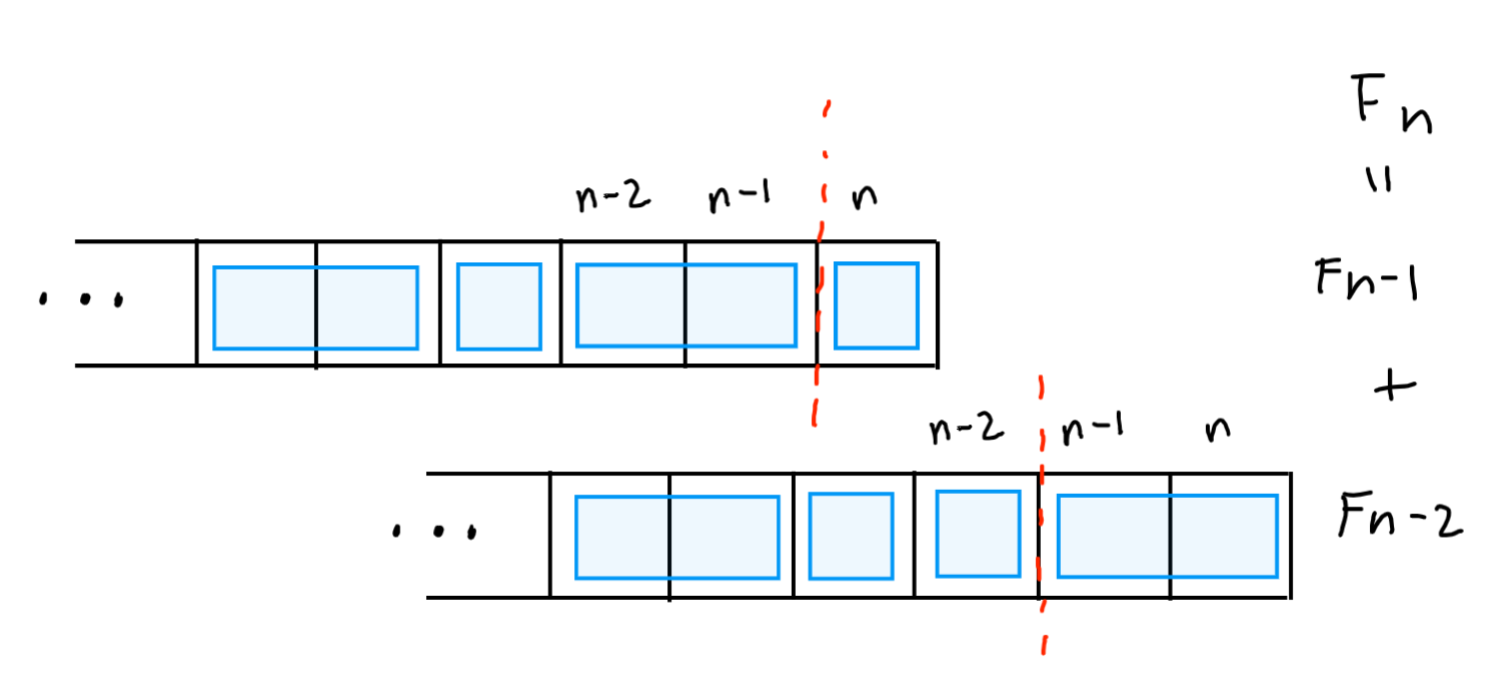
\includegraphics[width=4in]{1.png}
\end{center}
Now how do we force the recursion we want? We want to multiply the $F_{n-1}$ case with $x_n$. So that means we want $x_n$ possibilities if the last one is a square. The simplest way would be to require squares in the $n$th slot of the strip to have one of $1, 2, \ldots, x_n$ written on it. So the problem is now: how many ways are there to tile a $1 \times n$ strip with either squares or dominos, where a square on the $i$th slot needs to be labeled with one of $1, 2, \ldots, x_i$?

\begin{center}
\vspace{-0.5em}
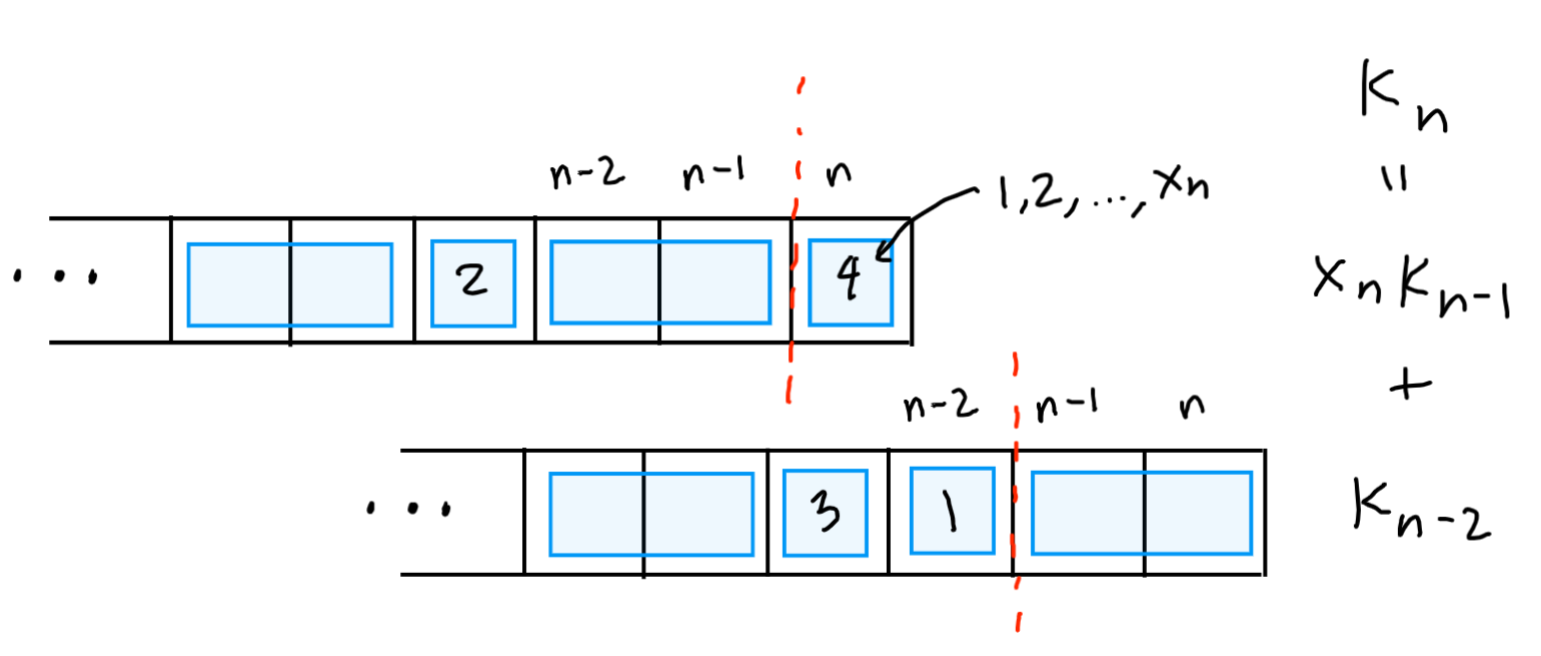
\includegraphics[width=4in]{2.png}
\end{center}

Well, let's say there are $K_n(x_1, \ldots, x_n)$ of them. There are two cases. If the last tile is a domino, the remaining tiles are a tiling of a $1 \times (n - 2)$ strip, and there are $K_{n-2}(x_1, \ldots, x_{n-2})$ ways to tile that. If the last tile is a square, it has $x_n$ possible labels, and for each label the remaining tiling is a $1 \times (n-1)$ strip, with $K_{n-1}(x_1, \ldots, x_{n-1})$ ways to tile that. Adding both cases together, we get the recursion \[
  K_n(x_1, \ldots, x_n) = x_n K_{n-1}(x_1, \ldots, x_{n-1}) + K_{n-2}(x_1, \ldots, x_{n-2}),
\]
as desired.

This allows us to show Euler's rule. Euler's rule says that we can find each term of $K_n(x_1, \ldots, x_n)$ by pairing up some consecutive $x_i$s and then multiplying the rest. For example, consider $K_4(x_1, \ldots, x_4)$:
\begin{itemthin}
\item If we pair nothing, we get the term $x_1x_2x_3x_4$.
\item If we pair $x_1$ and $x_2$, we get the term $x_3x_4$.
\item If we pair $x_1$ and $x_2$, and $x_3$ and $x_4$, we get the term $1$.
\item If we pair $x_2$ and $x_3$, we get the term $x_1x_4$.
\item If we pair $x_3$ and $x_4$, we get the term $x_1x_2$.
\end{itemthin}
Summing all the terms together indeed gives $K_4(x_1, \ldots, x_4)$. This comes directly from how we can count the number of tilings of the strip: placing the dominos is pairing up consecutive $x_i$s, then multiply the possibilities for the labels of the squares. This shows the \textbf{reversal identity}: \[
  K_n(x_1, \ldots, x_n) = K_n(x_n, \ldots x_1).
\]

\section{Bijections}

We can also use a bijection to prove that $K_n(x_1, \ldots, x_n) = K_n(x_n, \ldots x_1)$. The idea is to mirror the tiling. By doing so, we construct a one-to-one correspondence between the tilings on the left and the tilings on the right.

\begin{center}
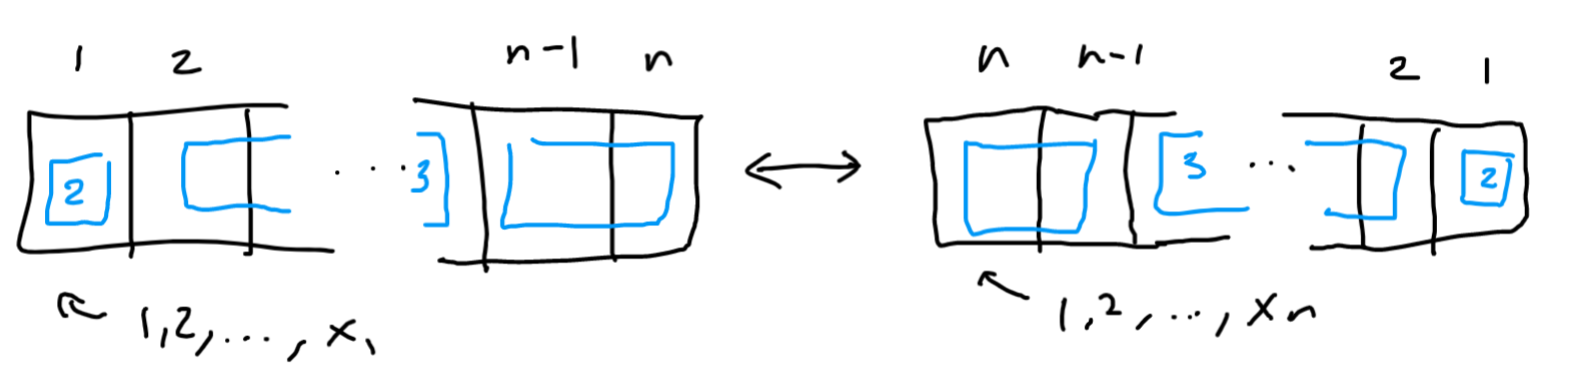
\includegraphics[width=4.5in]{3.png}
\end{center}

By using this reversal property for continued fractions, we get that
\begin{align*}
[a_1; a_2, \ldots, a_n] &=
\frac{K_n(a_1, \ldots, a_n)}{K_{n-1}(a_2, \ldots, a_n)} =
\frac{P_n}{Q_n} \\
\implies [a_n; a_{n-1}, \ldots, a_1] &=
\frac{K_n(a_n, \ldots, a_1)}{K_{n-1}(a_{n-1}, \ldots, a_1)} =
\frac{K_n(a_1, \ldots, a_n)}{K_{n-1}(a_1, \ldots, a_{n-1})}
= \frac{P_n}{P_{n-1}}.
\end{align*}
We can also try to prove $P_{n-1}Q_n - Q_{n-1}P_n = (-1)^{n-1}.$ Imagine a $1 \times n$ strip where a square on the $i$th slot needs to be labeled with $1, 2, \ldots, x_i$. Then the number of ways to tile this is $P_n$. Now imagine removing the first slot---so you have a $1 \times (n-1)$ strip where a square on the $i$th slot needs to be labeled with $1, 2, \ldots, x_{i+1}$. Then the number of ways to tile this is $Q_n$. We want to try to construct a one-to-one-ish correspondence between the tilings counted by $P_{n-1}Q_n$ and $Q_{n-1}P_n$.

Take a tiling counted in $P_{n-1}$ and a tiling counted in $Q_n$. These are both $1 \times (n-1)$ strips, except the maximum labels are shifted. Now look at the slices that can cut between the tiles. There's some slice that's can cut both tilings. Take the rightmost such slice, cut off the tiles at the end, and swap them. That gives a tiling counted by $P_n$ and a tiling counted by $Q_{n-1}$. This is easier explained with a picture.

\begin{center}
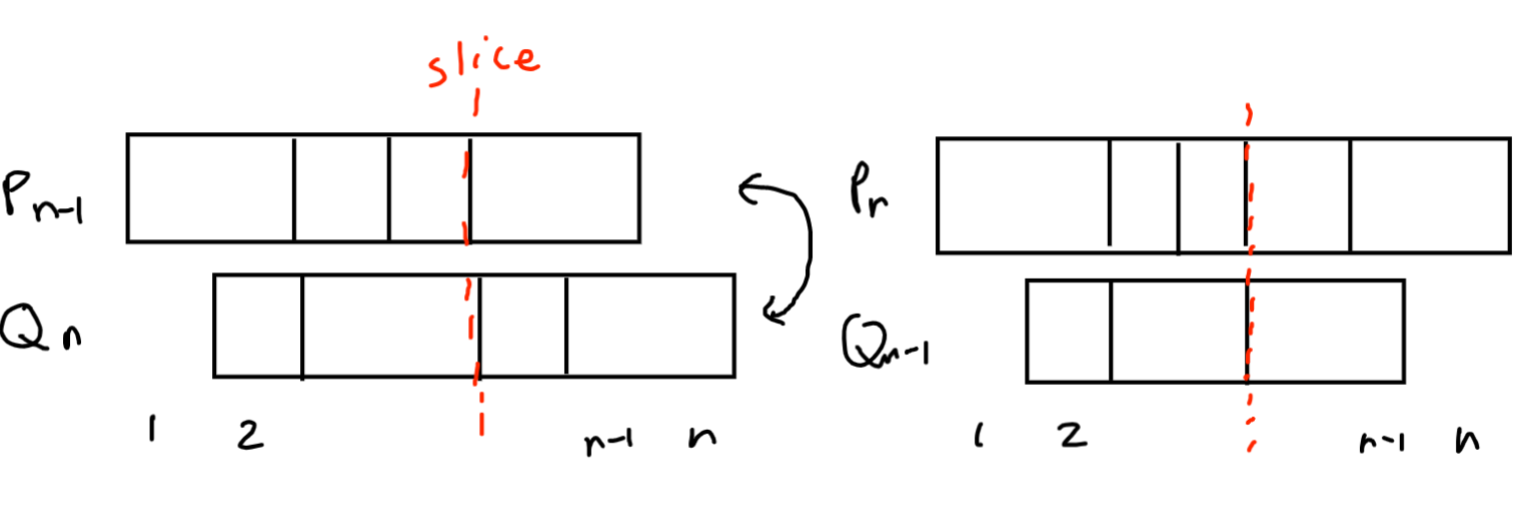
\includegraphics[width=4.5in]{4.png}
\end{center}

This is reversible, so the tilings counted are in bijection. Except! Except, there's always going to be exactly one case in which there's no such slice that cuts both tilings. It can only happen when both tilings consist of dominos that are arranged off-by-one. When $n$ is odd, this extra tiling is counted by $P_{n-1}Q_n$, and when $n$ is even, it's counted by $Q_{n-1}P_n$. This proves the identity.

\begin{center}
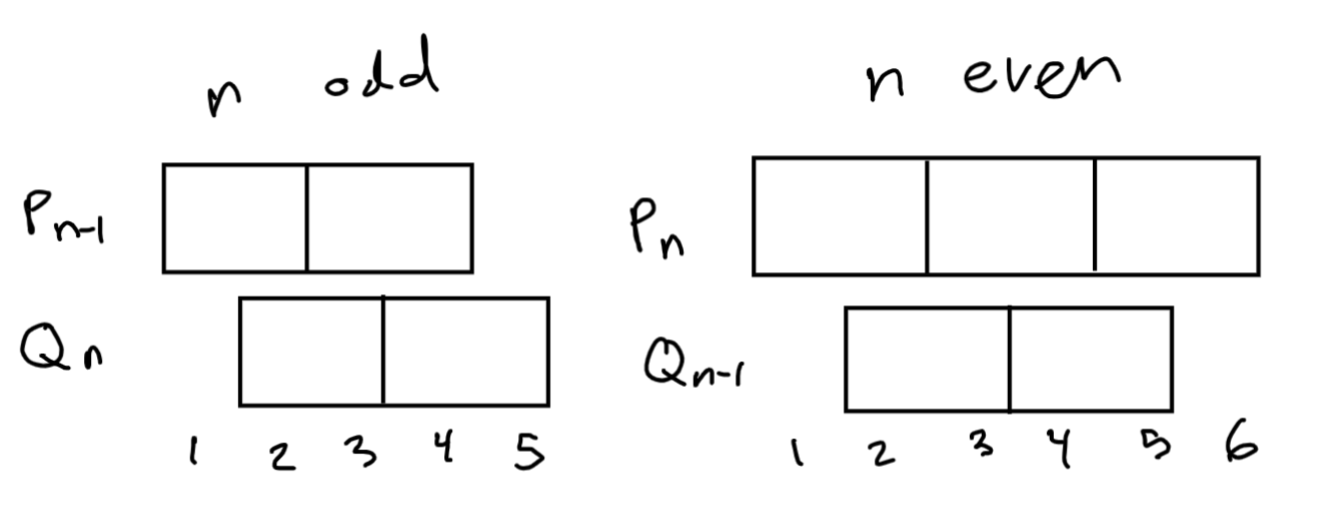
\includegraphics[width=4.5in]{5.png}
\end{center}

Similarly, we can prove $P_{n-2}Q_n - Q_{n-2}P_n = (-1)^na_n$ using a similar trick.

\begin{center}
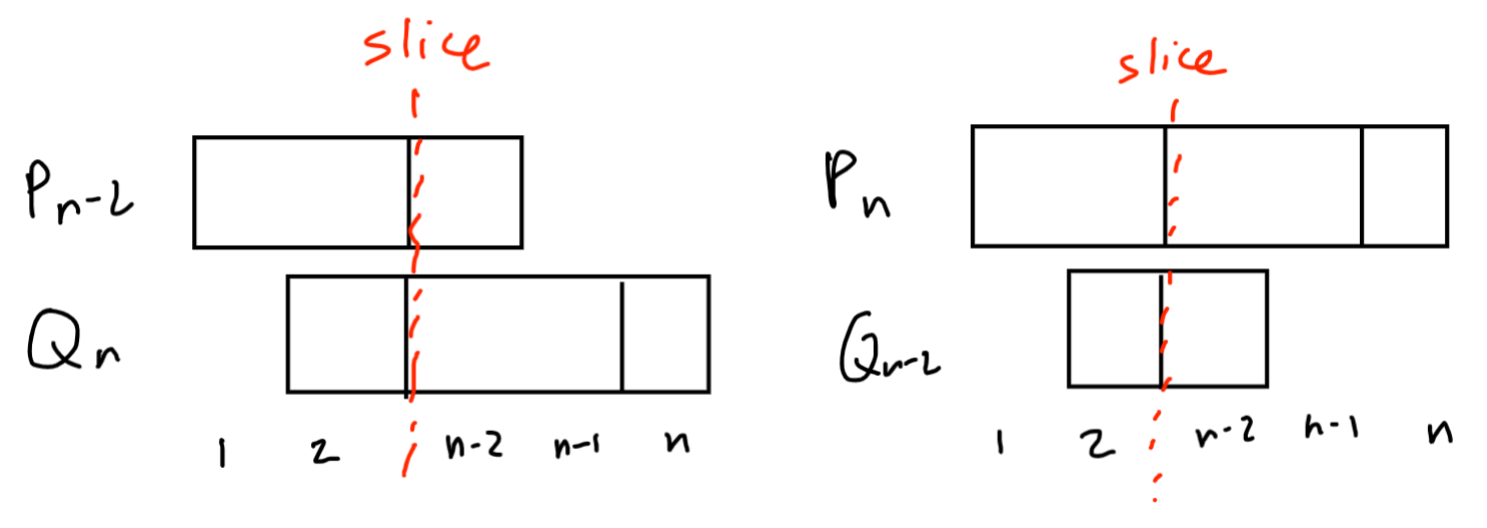
\includegraphics[width=4.5in]{6.png}
\end{center}

Which pairs of tilings don't have slices? It's gonna be all dominoes except for a final square. The final square has $a_n$ possible labels, and checking the parities gives the identity.

\begin{center}
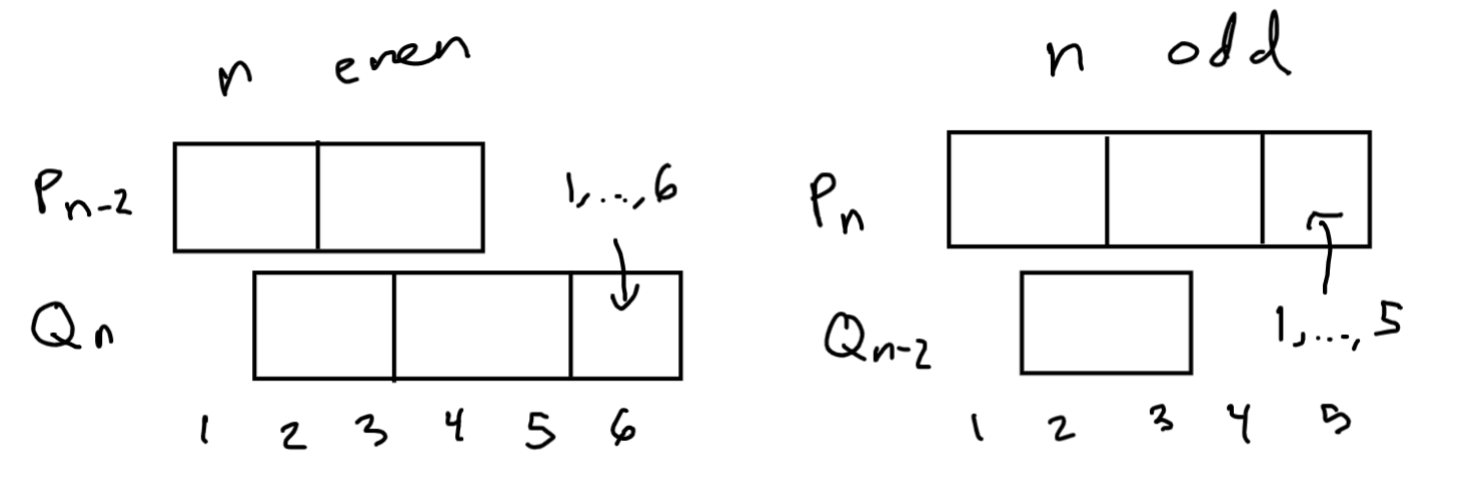
\includegraphics[width=4.5in]{7.png}
\end{center}

\section{Palindromes}

We'll now use the identities we've proven to show that every prime that's $1$ mod $4$ can be written as the sum of two squares, per \cite{benjamin2}. Okay, just kidding, we need one more identity. It's this one, which we'll call the \textbf{domino identity}: \[
  K_n(x_1, \ldots, x_n)
  = K_i(x_1, \ldots, x_i)K_{n-i}(x_{i+1}, \ldots, x_n)
  + K_{i-1}(x_1, \ldots, x_{i-1})K_{n-i-1}(x_{i+2}, \ldots, x_n).
\]
This one is also explained by our tiling interpretation. The right addend counts the cases where there is a domino in cells $i$ and $i+1$. The left addend counts the cases where there aren't.

Alright, now we go to the proof. Write $p = 4k + 1$. Consider the $2k - 1$ continued fractions of \[
  \frac{p}{2}, \frac{p}{3}, \dots, \frac{p}{2k}.
\]
Consider the continued fractions for each of them, say $\frac{p}{i} = [a_1; \ldots, a_n]$. Because $i \le 2k < p/2$, we get $a_1 \ge 2$. Further, because of the convention that we listed in the very beginning, $a_n \ge 2$ as well. (If it wasn't, we just combine it with $a_{n-1}$.) Now reverse its continued fraction to get $[a_n; \ldots, a_1]$. We know from a previous result that its numerator has to be $p$. We also know, because $a_n \ge 2$, that its denominator has to be at most $2k$. So $[a_n; \ldots, a_1]$ is one of the $2k - 1$ fractions we listed above.

The process of reversing the continued fractions pairs up the $2k - 1$ fractions we listed. Because $2k - 1$ is odd, it follows there exists some fraction \[
  \frac{p}{i} = [a_1; \ldots, a_n] = [a_n; \ldots, a_1].
\]
So there's some palindromic continued fraction. There are two cases, whether $n$ is odd or even:
\begin{itemize}
\item The continued fraction is $[a_1; \ldots, a_m, a_{m+1}, a_m, \ldots, a_1]$. Then the numerator is
\begin{align*}
p &= K_n(a_1, \ldots, a_m, a_{m+1}, a_m, \ldots, a_1) \\
&= K_m(a_1, \ldots, a_m)K_{m+1}(a_{m+1}, \ldots, a_1)
+ K_{m-1}(a_1, \ldots, a_{m-1})K_{m}(a_m, \ldots, a_1) \\
&= K_m(a_1, \ldots, a_m)K_{m+1}(a_{m+1}, \ldots, a_1)
+ K_{m-1}(a_1, \ldots, a_{m-1})K_{m}(a_1, \ldots, a_m) \\
&= K_m(a_1, \ldots, a_m) \left(
K_{m+1}(a_{m+1}, \ldots, a_1)
+ K_{m-1}(a_1, \ldots, a_{m-1})
\right).
\end{align*}
From the top, we used the domino identity, then the reversal identity, then we factored. As $a_1 \ge 2$, both factors are integers that are at least $2$. Hence $p$ is composite, contradiction.

\item The continued fraction is $[a_1; \ldots, a_m, a_m, \ldots, a_1]$. Then the numerator is
\begin{align*}
p &= K_n(a_1, \ldots, a_m, a_m, \ldots, a_1) \\
&= K_m(a_1, \ldots, a_m)K_m(a_m, \ldots, a_1)
+ K_{m-1}(a_1, \ldots, a_{m-1})K_{m-1}(a_{m-1}, \ldots, a_1) \\
&= K_m(a_1, \ldots, a_m)^2 + K_{m-1}(a_1, \ldots, a_{m-1})^2.
\end{align*}
Once again, we used the domino identity, then the reversal identity. This shows that $p$ is the sum of two squares, as desired!
\end{itemize}

\section{A magic trick}

We begin with a magic trick, per \cite{bah}. An interesting fact about the continued fraction of $\sqrt{n}$, for an integer $n$, is that not only periodic, but kinda palindromic, where the last coefficient is twice the first one. For example, we can compute \[
  \sqrt{1271} = [35; \ol{1, 1, 1, 6, 2, 6, 1, 1, 1, 70}].
\]
Now here is the magic trick. Split the periodic part in half: $1, 1, 1, 6, 2$ and $6, 1, 1, 1, 70$. Swap them to get the new periodic half, $\ol{6, 1, 1, 1, 70, 1, 1, 1, 6, 2}$. Now halve the last coefficient of the periodic half to form a new continued fraction, $[1; \ol{6, 1, 1, 1, 70, 1, 1, 1, 6, 2}]$. A computation followed by the quadratic formula shows us that this is $\sqrt{\frac{41}{31}}$. And magically enough, $1271 = 41 \cdot 31$.

This trick works only when the period is even and when the thing you have to halve is also even. It also only works when the thing you're taking the square root of is a product of two squarefree integers. But when it does work, it's pretty cool. Here's an explanation, per \cite{spier}.

First we need two identities. The first one follows from subtracting the recursive definitions of two continuants:
\begin{align*}
K_n(x_1, \ldots, x_n + d) &=
(x_n + d)K_{n-1}(x_1, \ldots, x_{n-1})
+ K_{n-2}(x_1, \ldots, x_{n-2}) \\
K_n(x_1, \ldots, x_n) &=
x_n K_{n-1}(x_1, \ldots, x_{n-1})
+ K_{n-2}(x_1, \ldots, x_{n-2}) \\
K_n(x_1, \ldots, x_n + d) - K_n(x_1, \ldots, x_n)
&= d K_{n-1}(x_1, \ldots, x_{n-1}).
\end{align*}
The second identity is: \[
K_{2n+1}(x_1, \ldots, x_n, 2x_{n+1}, x_n, \ldots, x_1)
= 2K_n(x_1, \ldots, x_n)K_{n+1}(x_1, \ldots, x_{n+1}).\]
This one follows from a counting argument. Take a tiling counted by the left side. If there's a domino covering the $n+1$st slot, cut along its boundary to produce a strip of length $n$ and a strip of length $n+1$; this gets counted by the right side. This is reversible in exactly two ways: either we put the strip of length $n+1$ before $n$, or $n$ before $n+1$.

\begin{center}
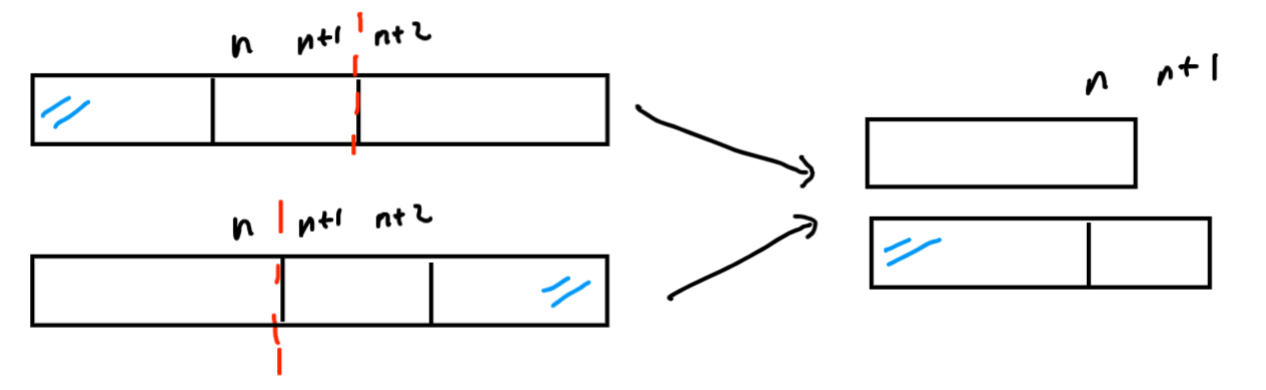
\includegraphics[width=5in]{8.png}
\end{center}

Now suppose there isn't a domino covering the $n+1$st slot. It's tiled by a square with label $x$. If $x$ is even, cut between the $n$th and $n+1$st slot; if $x$ is odd, cut between the $n+1$st and $n+2$nd slot. Then change the label of the $n+1$st slot to $\ceil{\frac{x}{2}}$. This way the new middle tile fits the bounds for its label. This is again reversible in exactly two ways.

\begin{center}
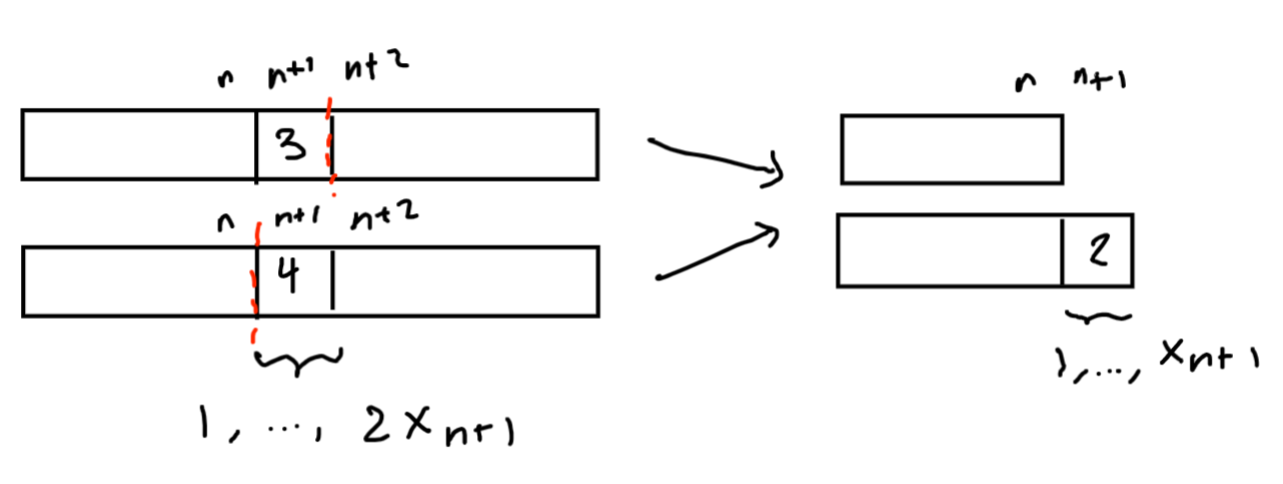
\includegraphics[width=5in]{9.png}
\end{center}

And now for the proof! Let's say \[
  x = [a_1; \ol{a_2, \ldots, a_m, 2a_{m+1}, a_m, \ldots, 2a_1}].
\]
Then
\begin{align*}
x &= [a_1; a_2, \ldots, a_m, 2a_{m+1}, a_m, \ldots, a_1 + x] \\
x &= \frac{K_{2m+1}(a_1, \ldots, a_2, a_1 + x)}{K_{2m}(a_2, \ldots, a_2, a_1 + x)} \\
x &= \frac{x K_{2m}(a_1, \ldots, a_2) + K_{2m+1}(a_1, \ldots, a_2, a_1)}{x K_{2m-1}(a_2, \ldots, a_2) + K_{2m}(a_2, \ldots, a_2, a_1)} \\
x^2 K_{2m-1}(a_2, \ldots, a_2) &= K_{2m+1}(a_1, \ldots, a_2, a_1) \\
x &= \sqrt{\frac{K_{2m+1}(a_1, \ldots, a_m, 2a_{m+1}, a_m, \ldots, a_1)}{K_{2m-1}(a_2, \ldots, a_m, 2a_{m+1}, a_m, a_2)}} \\
x &= \sqrt{\frac{2K_m(a_1, \ldots, a_m)K_{m+1}(a_1, \ldots, a_{m+1})}{2K_{m-1}(a_2, \ldots, a_m)K_m(a_2, \ldots, a_{m+1})}}.
\end{align*}
Now swap the $K_m(a_1, \ldots, a_m)$ and $K_m(a_2, \ldots, a_{m+1})$ between the numerator and denominator. This represents the switch from $\sqrt{pq}$ to $\sqrt{\frac{p}{q}}$. Showing that there's a divisibility here, that $p$ and $q$ are actually integers, is a bit more complicated, see \cite{van}. But anyway:
\begin{align*}
y &= \sqrt{\frac{2K_m(a_2, \ldots, a_{m+1})K_{m+1}(a_1, \ldots, a_{m+1})}{2K_{m-1}(a_2, \ldots, a_m)K_m(a_1, \ldots, a_m)}}.
\end{align*}
Then use the reversal identity to reverse all the continuants, and follow the steps backwards to get \[
  y = [a_{m+1}, \ol{a_m, \ldots, a_2, 2a_1, a_2, \ldots, 2a_{m+1}}].
\]

\section{Generalizations}

Here's one nice generalization. Generalize the continuants to depend on \emph{two sequences} $a_1, \ldots, a_n$ and $b_1, \ldots, b_{n-1}$, so that
\begin{align*}
K_0 &= 1 \\
K_1 &= a_1 \\
K_n &= a_n K_{n-1} + b_{n-1} K_{n-2}.
\end{align*}
Observe that these can be counted with tilings of a $1 \times n$ strip, where squares on the $i$th slot need to be labeled with $1, \ldots, a_i$, and dominos on the $i$th and $i+1$st slots need to be labeled with $1, \ldots, b_i$. So, same thing as previous, but with dominos labeled too. The fun fact is that $K_n$ is the $n$th convergent of the generalized continued fraction \[
  a_1 + \cfrac{b_1}{
    a_2 + \cfrac{b_2}{
      \ddots + \cfrac{b_{k-1}}{a_k}
    }
  },
\]
where we cut off the fraction at $\frac{b_{n-1}}{a_n}$ to get the $n$th convergent. This also generalizes with the matrices, e.g. \[
  K_n
  = \det\bm{
  a_1 & b_1 & 0 & \cdots & 0 & 0 \\
  -1 & a_2 & b_2 & \cdots & 0 & 0 \\
  0 & -1 & \ddots& \ddots & \vdots & \vdots \\
  \vdots & \vdots & \ddots & a_{n-2} & b_{n-2} & 0 \\
  0 & 0 & \cdots & -1 & a_{n-1} & b_{n-1} \\
  0 & 0 & \cdots & 0 & -1 & a_n
  }.
\]
Can you prove these? Can you generalize even further?

\begin{thebibliography}{99}
  \bibitem{bah} bah. Why does this continued fraction factorization magic trick work? \url{https://math.stackexchange.com/a/3701286/680415}

  \bibitem{benjamin1} Benjamin, A. T., Su, F. E., Quinn, J. J. Counting on Continued Fractions. \url{https://www.jstor.org/stable/pdf/2691080.pdf}

  \bibitem{benjamin2} Benjamin, A. T., Zeilberger, D. Pythagorean Primes and Palindromic Continued Fractions. \url{https://www.emis.de/journals/INTEGERS/papers/f30/f30.pdf}

  \bibitem{booher} Booher, J. Continued Fractions, Pell's Equation, and Transcendental Numbers. \url{https://www.math.canterbury.ac.nz/~j.booher/expos/continued_fractions.pdf}

  \bibitem{spier} Spier, T. J. On Means of Near Continued Fractions. \url{https://arxiv.org/pdf/2005.07181.pdf}

  \bibitem{van} van der Poorten, A. J., Walsh, P. G. A Note on Jacobi Symbols and Continued Fractions. \url{https://www.tandfonline.com/doi/pdf/10.1080/00029890.1999.12005008}
\end{thebibliography}

If you spot a typo, see an error, have a suggestion, or want to ask a question, feel free to contact me at \mailto{cj@cjquines.com}.

\end{document}
